% Created by tikzDevice version 0.12.3.1 on 2021-07-04 20:35:17
% !TEX encoding = UTF-8 Unicode
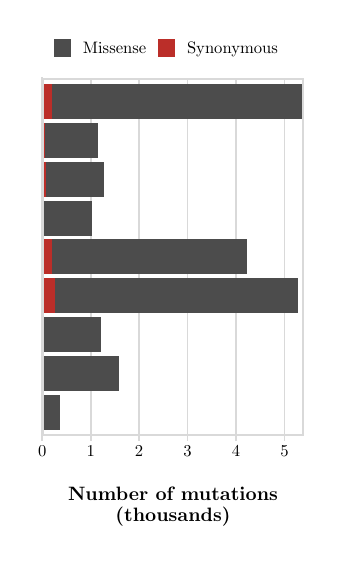
\begin{tikzpicture}[x=1pt,y=1pt]
\definecolor{fillColor}{RGB}{255,255,255}
\path[use as bounding box,fill=fillColor,fill opacity=0.00] (0,0) rectangle (103.28,183.39);
\begin{scope}
\path[clip] (  5.25, 35.86) rectangle ( 99.78,165.19);
\definecolor{drawColor}{gray}{0.85}

\path[draw=drawColor,line width= 0.6pt,line join=round] (  5.25, 35.86) --
	(  5.25,165.19);

\path[draw=drawColor,line width= 0.6pt,line join=round] ( 22.77, 35.86) --
	( 22.77,165.19);

\path[draw=drawColor,line width= 0.6pt,line join=round] ( 40.28, 35.86) --
	( 40.28,165.19);

\path[draw=drawColor,line width= 0.6pt,line join=round] ( 57.80, 35.86) --
	( 57.80,165.19);

\path[draw=drawColor,line width= 0.6pt,line join=round] ( 75.31, 35.86) --
	( 75.31,165.19);

\path[draw=drawColor,line width= 0.6pt,line join=round] ( 92.83, 35.86) --
	( 92.83,165.19);
\definecolor{fillColor}{gray}{0.30}

\path[fill=fillColor] (  8.74,150.43) rectangle ( 99.78,163.08);
\definecolor{fillColor}{RGB}{187,46,41}

\path[fill=fillColor] (  5.25,150.43) rectangle (  8.74,163.08);
\definecolor{fillColor}{gray}{0.30}

\path[fill=fillColor] (  6.25,136.37) rectangle ( 25.25,149.02);
\definecolor{fillColor}{RGB}{187,46,41}

\path[fill=fillColor] (  5.25,136.37) rectangle (  6.25,149.02);
\definecolor{fillColor}{gray}{0.30}

\path[fill=fillColor] (  6.56,122.31) rectangle ( 27.44,134.97);
\definecolor{fillColor}{RGB}{187,46,41}

\path[fill=fillColor] (  5.25,122.31) rectangle (  6.56,134.97);
\definecolor{fillColor}{gray}{0.30}

\path[fill=fillColor] (  5.25,108.26) rectangle ( 23.22,120.91);

\path[fill=fillColor] (  8.93, 94.20) rectangle ( 79.36,106.85);
\definecolor{fillColor}{RGB}{187,46,41}

\path[fill=fillColor] (  5.25, 94.20) rectangle (  8.93,106.85);
\definecolor{fillColor}{gray}{0.30}

\path[fill=fillColor] (  9.87, 80.14) rectangle ( 97.73, 92.79);
\definecolor{fillColor}{RGB}{187,46,41}

\path[fill=fillColor] (  5.25, 80.14) rectangle (  9.87, 92.79);
\definecolor{fillColor}{gray}{0.30}

\path[fill=fillColor] (  5.81, 66.09) rectangle ( 26.62, 78.74);
\definecolor{fillColor}{RGB}{187,46,41}

\path[fill=fillColor] (  5.25, 66.09) rectangle (  5.81, 78.74);
\definecolor{fillColor}{gray}{0.30}

\path[fill=fillColor] (  5.25, 52.03) rectangle ( 32.87, 64.68);

\path[fill=fillColor] (  5.43, 37.97) rectangle ( 11.78, 50.62);
\definecolor{fillColor}{RGB}{187,46,41}

\path[fill=fillColor] (  5.25, 37.97) rectangle (  5.43, 50.62);

\path[draw=drawColor,line width= 1.1pt,line join=round,line cap=round] (  5.25, 35.86) rectangle ( 99.78,165.19);
\end{scope}
\begin{scope}
\path[clip] (  0.00,  0.00) rectangle (103.28,183.39);
\definecolor{drawColor}{gray}{0.85}

\path[draw=drawColor,line width= 0.6pt,line join=round,line cap=rect] (  5.25, 35.86) --
	(  5.25,165.19);
\end{scope}
\begin{scope}
\path[clip] (  0.00,  0.00) rectangle (103.28,183.39);
\definecolor{drawColor}{gray}{0.85}

\path[draw=drawColor,line width= 0.6pt,line join=round] (  5.25, 34.11) --
	(  5.25, 35.86);

\path[draw=drawColor,line width= 0.6pt,line join=round] ( 22.77, 34.11) --
	( 22.77, 35.86);

\path[draw=drawColor,line width= 0.6pt,line join=round] ( 40.28, 34.11) --
	( 40.28, 35.86);

\path[draw=drawColor,line width= 0.6pt,line join=round] ( 57.80, 34.11) --
	( 57.80, 35.86);

\path[draw=drawColor,line width= 0.6pt,line join=round] ( 75.31, 34.11) --
	( 75.31, 35.86);

\path[draw=drawColor,line width= 0.6pt,line join=round] ( 92.83, 34.11) --
	( 92.83, 35.86);
\end{scope}
\begin{scope}
\path[clip] (  0.00,  0.00) rectangle (103.28,183.39);
\definecolor{drawColor}{RGB}{0,0,0}

\node[text=drawColor,anchor=base,inner sep=0pt, outer sep=0pt, scale=  0.60] at (  5.25, 28.48) {0};

\node[text=drawColor,anchor=base,inner sep=0pt, outer sep=0pt, scale=  0.60] at ( 22.77, 28.48) {1};

\node[text=drawColor,anchor=base,inner sep=0pt, outer sep=0pt, scale=  0.60] at ( 40.28, 28.48) {2};

\node[text=drawColor,anchor=base,inner sep=0pt, outer sep=0pt, scale=  0.60] at ( 57.80, 28.48) {3};

\node[text=drawColor,anchor=base,inner sep=0pt, outer sep=0pt, scale=  0.60] at ( 75.31, 28.48) {4};

\node[text=drawColor,anchor=base,inner sep=0pt, outer sep=0pt, scale=  0.60] at ( 92.83, 28.48) {5};
\end{scope}
\begin{scope}
\path[clip] (  0.00,  0.00) rectangle (103.28,183.39);
\definecolor{drawColor}{RGB}{0,0,0}

\node[text=drawColor,anchor=base,inner sep=0pt, outer sep=0pt, scale=  0.70] at ( 52.51, 12.42) {\bfseries Number of mutations};

\node[text=drawColor,anchor=base,inner sep=0pt, outer sep=0pt, scale=  0.70] at ( 52.51,  4.86) {\bfseries (thousands)};
\end{scope}
\begin{scope}
\path[clip] (  0.00,  0.00) rectangle (103.28,183.39);
\definecolor{fillColor}{gray}{0.30}

\path[fill=fillColor] (  9.46,172.90) rectangle ( 15.74,179.18);
\end{scope}
\begin{scope}
\path[clip] (  0.00,  0.00) rectangle (103.28,183.39);
\definecolor{fillColor}{RGB}{187,46,41}

\path[fill=fillColor] ( 47.10,172.90) rectangle ( 53.37,179.18);
\end{scope}
\begin{scope}
\path[clip] (  0.00,  0.00) rectangle (103.28,183.39);
\definecolor{drawColor}{RGB}{0,0,0}

\node[text=drawColor,anchor=base west,inner sep=0pt, outer sep=0pt, scale=  0.60] at ( 19.95,173.97) {Missense};
\end{scope}
\begin{scope}
\path[clip] (  0.00,  0.00) rectangle (103.28,183.39);
\definecolor{drawColor}{RGB}{0,0,0}

\node[text=drawColor,anchor=base west,inner sep=0pt, outer sep=0pt, scale=  0.60] at ( 57.58,173.97) {Synonymous};
\end{scope}
\end{tikzpicture}
